\chapter{Desarrollo}
Recordemos de la Figura \ref{fig:diagrama_bloques_objetivo} que nuestro sistema está compuesto por 5 bloques. En este capítulo vamos descomponer y analizar cada bloque para su posterior implementación en la simulación.

\section{Análisis}
\subsection*{Codificador y Modulador}
Estos bloques son en realidad bastante simples. Consta de la sumatoria de dos señales sinusoidales. Para la simulación serían dos generadores establecidos en la combinación de frecuencias que corresponden a un determinado digito. Para crear la codificación, basta con ingresar ambas señales a un sumador. Esto luego debe sumarse a una señal constante de 1, con el fin de poder hacer el producto de la señal resultante con la señal portadora. El resultado de esto es la señal ya modulada, como se muestra en la Figura \ref{fig:bloques_cod_mod}.

\begin{figure}[H]
  \centering
  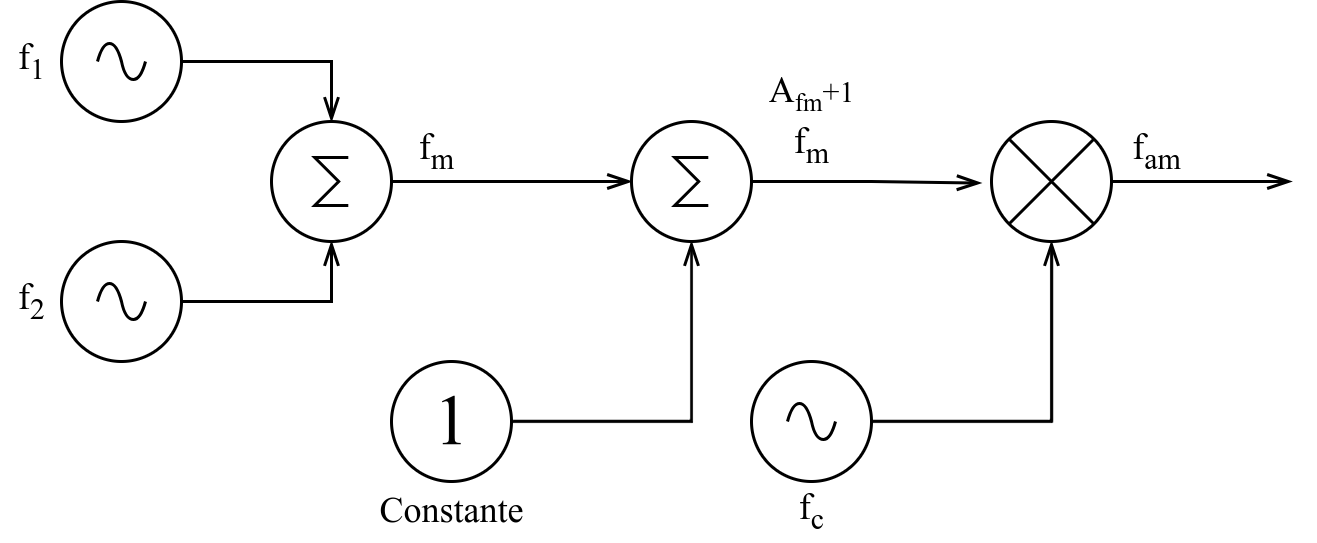
\includegraphics[width=400pt]{images/diagramas-codificador-modulador.png}
  \caption{Codificador y Modulador}
  \label{fig:bloques_cod_mod}
\end{figure}

\subsection*{Transmisión}
La transmisión será simulada a través de un filtro pasa-banda, estableciendo las frecuencias de corte de tal forma que el ancho de banda sea el espectro audible por el oído humano, como muestra la Figura \ref{fig:bloques_txs}.

\begin{figure}[H]
  \centering
  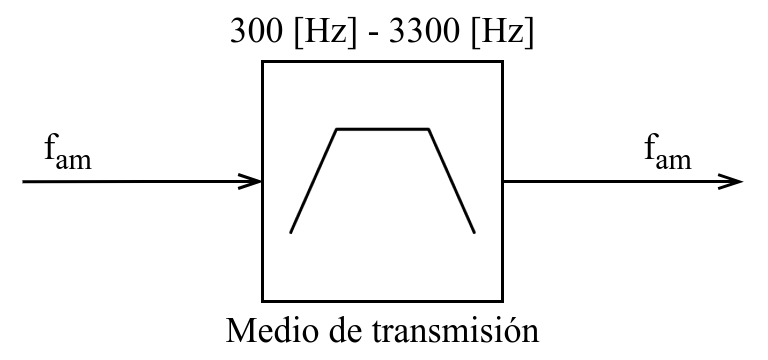
\includegraphics[width=300pt]{images/diagramas-transmision.png}
  \caption{Transmisión}
  \label{fig:bloques_txs}
\end{figure}

\subsection*{Demodulador}
Para demodular la señal, basta con realizar nuevamente el producto con la señal portadora. Como resultado obtenemos la frecuencia moduladora (que es la señal codificada, suma de las frecuencias que componen a un digito específico) como muestra la Figura \ref{fig:bloques_demod}. Luego debemos aplicar un filtro pasa bajos para limpiar la señal de ruidos que puedan haberse introducido, entre esos, algunos vestigios de la señal portadora.

\begin{figure}[H]
  \centering
  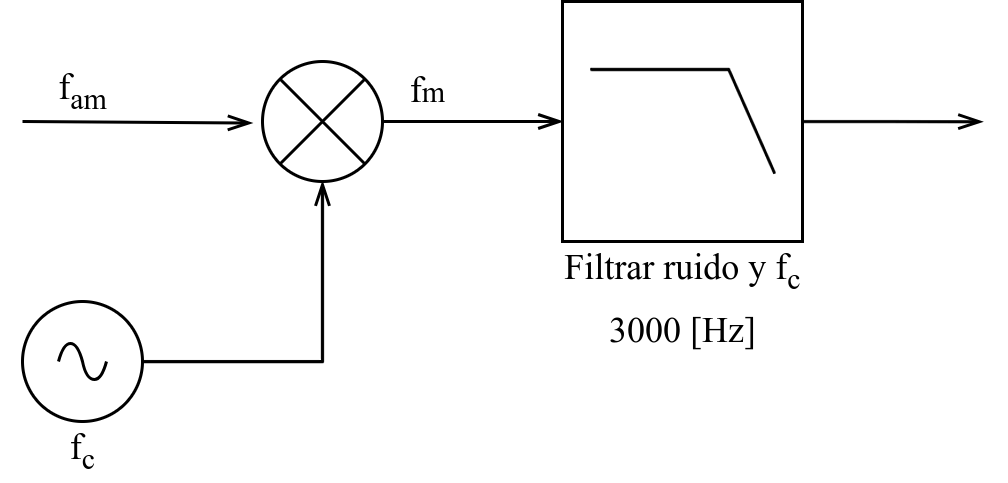
\includegraphics[width=350pt]{images/diagramas-demodulador.png}
  \caption{Transmisión}
  \label{fig:bloques_demod}
\end{figure}

\subsection*{Decodificador}
El bloque decodificador es el más complejo de todos, ya que este tiene la lógica para detectar las señales que componen la señal codificada. Como ya vimos en la Figura \ref{fig:diagrama_bloques_decod}, necesitamos 7 filtros pasa-banda para aislar cada una de las frecuencias de la matriz \gls{dtfm}, luego viene la matriz decodificadora. En la Figura \ref{fig:bloques_decod} vemos una simplificación de cómo estaría compuesta esta lógica de decodificación. Cada salida de control es una compuerta AND que se activara cuando sus dos entradas se encuentren activas (o en "1" lógico). Entonces cada compuerta representa la combinación de tonos para detectar cuál fué el digito enviado.

\begin{figure}[H]
  \centering
  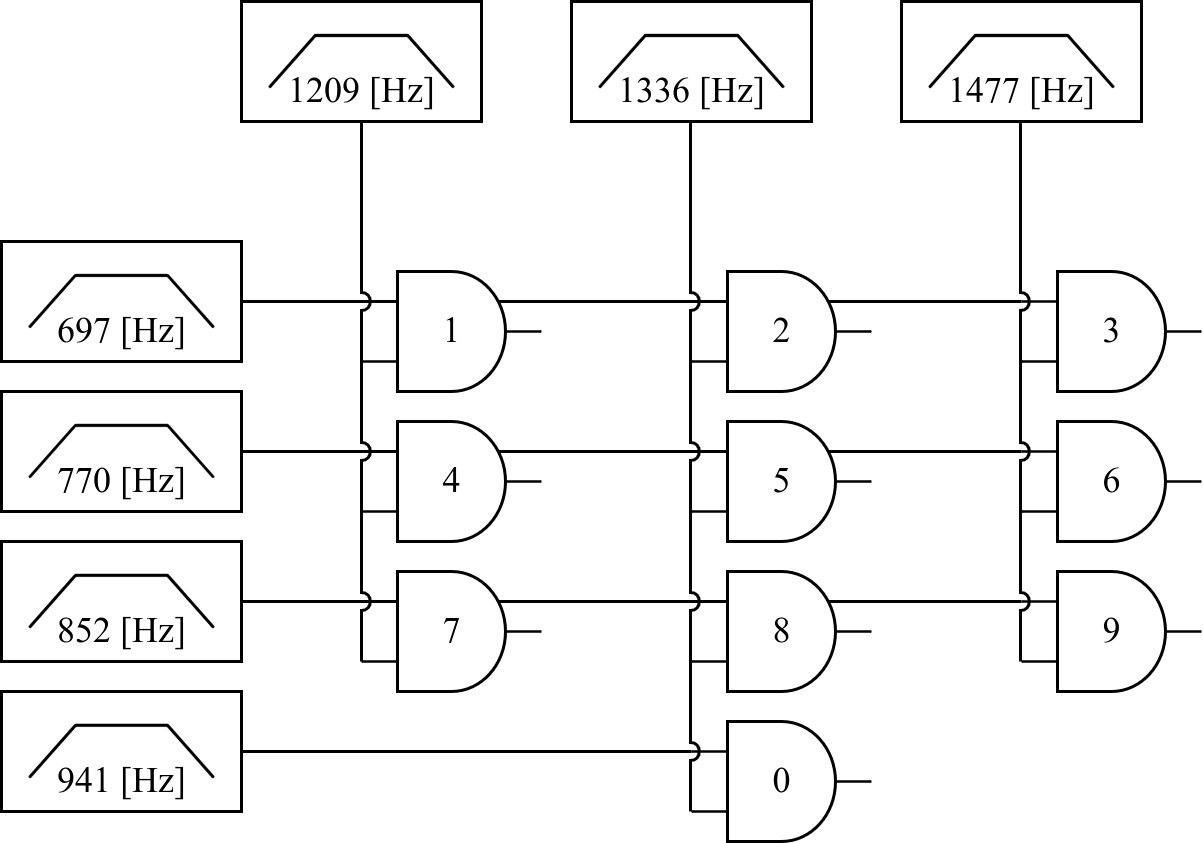
\includegraphics[width=350pt]{images/diagramas-decodificador-matriz.png}
  \caption{Decodificador}
  \label{fig:bloques_decod}
\end{figure}

\section{Diseño}
Como mencionamos en la sección anterior, para poder implementar los filtros digitales del banco de filtros (bloque decodificador) necesitamos librerías de MATLAB para generarlos, ya que estos filtros serán de alto orden lo que es engorroso para el cálculo analítico. Para hacer uso de estas librerías se crearon 2 \textit{scripts} con el objetivo de automatizar la generación de los filtros en base a parámetros de entrada. En el Código \ref{code:banco_decodificador} podemos ver que se encarga de calcular las frecuecias de corte (inferior y superior) para cada frecuencia central provista, bajo una determinada frecuencia de muestreo y orden específico, esto para el banco de filtros del decodificador. Además de eso, también podemos ver que genera las gráficas para analizar la respuesta en frecuencia de cada filtro, como muestra la Figura \ref{fig:banco_filtros_resp_frec}. Luego en el Código \ref{code:algoritmo_principal} tenemos el algorítmo principal, el cual establece las especificaciones generales del sistema, llama a la función para crear el banco de filtros y además crea el resto de los filtros involucrados como el que representa el canal de transmición y el filtro para eleminar la portadora del espectro de trabajo (en la fase de demodulación).

Se puede notar en el Código \ref{code:algoritmo_principal} que establecemos el orden de los filtros en 6 (para pasa-bajos y/o pasa-altos; se interpreta 12 para pasa-banda). Este valor arbitrario, contrario a los cálculos analíticos del capítulo anterior, es empírico; durante varias pruebas de simulación, los filtros pasa-banda de alto orden (20 aproximadamente) demostraban comportamientos inesperados y no concluyentes a la hora de filtrar señales específicas. Por eso, luego de varias pruebas encontramos que el orden 6 era suficiente para realizar la simulación con resultados favorables y realistas.

\begin{figure}[H]
  \lstinputlisting[
    language=Octave,
    caption={Banco Decodificador},
    label={code:banco_decodificador}
  ]{matlab/banco_decodificador.m}
\end{figure}

\begin{figure}[H]
  \centering
  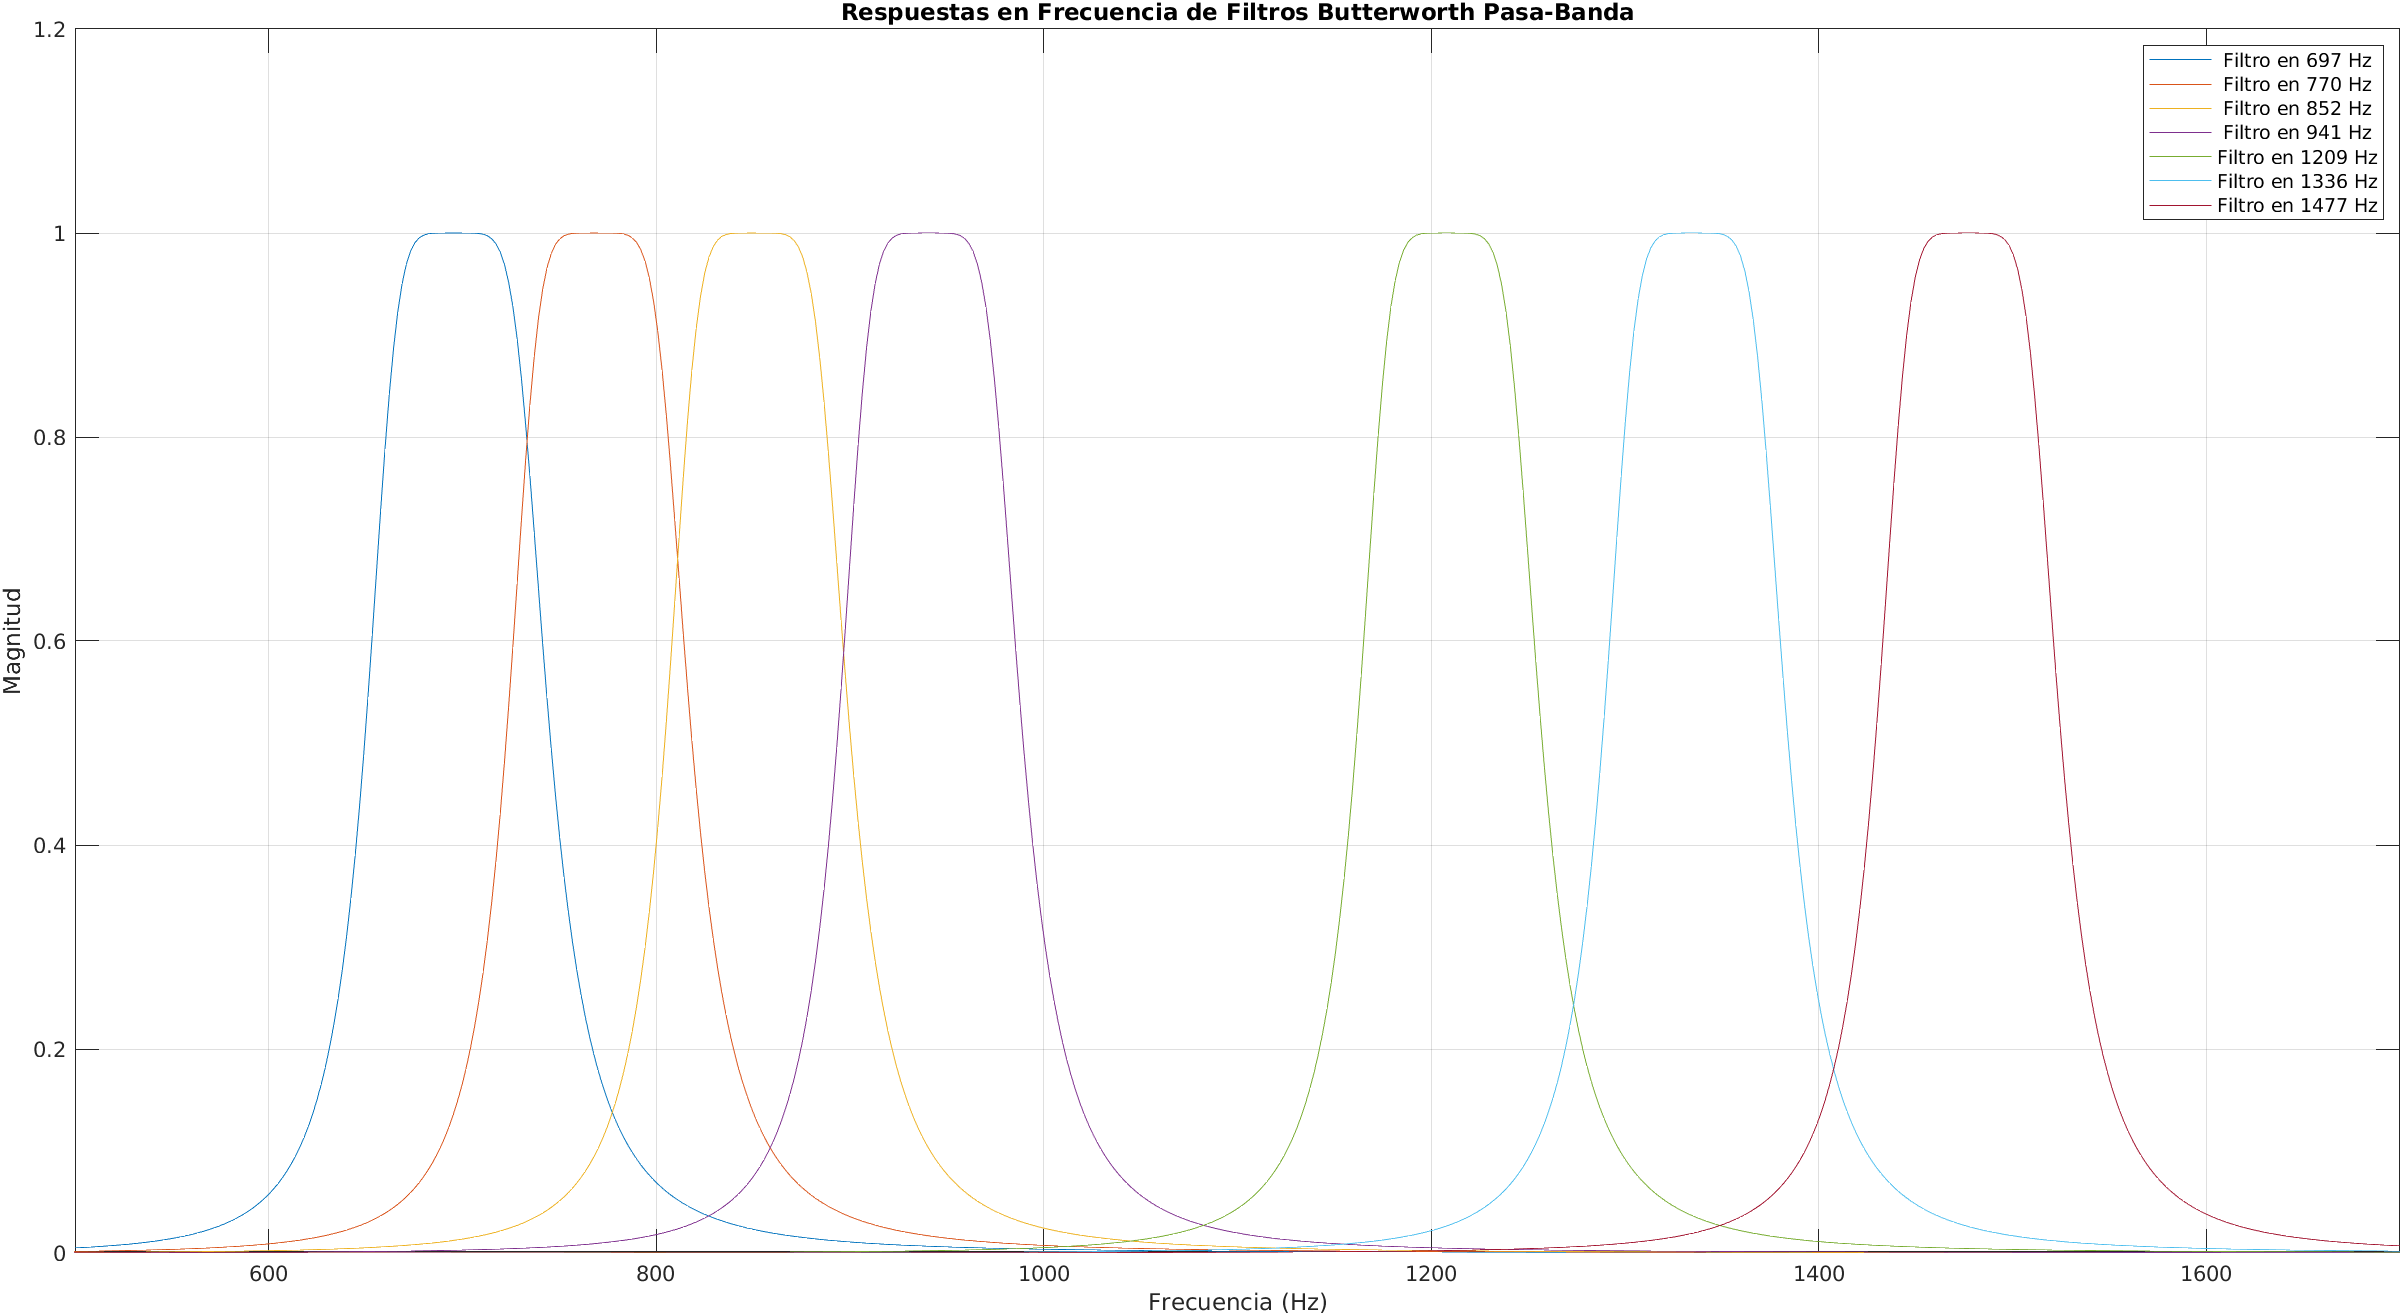
\includegraphics[width=\linewidth]{images/resp_frec_banco_filtros.png}
  \caption{Respuesta en frecuencia del Banco de Filtros}
  \label{fig:banco_filtros_resp_frec}
\end{figure}

\begin{figure}[H]
  \lstinputlisting[
    language=Octave,
    caption={Algorítmo principal},
    label={code:algoritmo_principal}
  ]{matlab/main.m}
\end{figure}

\section{Prototipo}
En base a los resultados obtenidos de los \textit{scripts} diseñamos el sistema completo, en los que cada bloque se alimenta de los datos resultantes. En la Figura \ref{fig:bloques_modem} podemos ver los bloques intervinientes en la primera parte del sistema, esta incluye la selección de los tonos (inferior y superior) para luego sumarlos y lograr la codificación \gls{dtfm} del número 5 en este caso. Luego pasamos a los bloques intervinientes en la modulación AM de las señales, sumando antes una constante 1 para poder realizar el producto con la señal portadora. Una vez obtenida la señal modulada en AM, esta se transmite por el canal de modulación, que según las especificaciones tiene el ancho de banda del espectro audible por el oído humano. Luego llega a la etapa de demodulación, en la que la señal se vuelve a batir (producto) con la portadora, y el resultado es una señal que tiene una componente en la frecuencia de la portadora y debe ser filtrada, por ello utilizamos un filtro pasa-bajos con frecuencia de corte 3[kHz]. Pasado este filtro, la señal obtenida es casi identica a la sumatoria de los dos tonos.

La segunda parte del sistema comprende la decodificación \gls{dtfm} a través de un banco de filtros y una matriz decodificadora, como se muestra en la Figura \ref{fig:bloques_codec}. Primero debemos aislar las señales por tonos diferenciados, esto lo hace el banco de filtros digitales. Cada uno de estos es un filtro pasa-banda con frecuencia central en uno de los 7 tonos, de esta forma logramos aislar cada señal. Dado que estas son sinusoidales, necesitamos calcular el valor efectivo de las mismas para poder operar lógicamente ellas, entonces se coloca un bloque que realiza el cálculo. Luego, el valor obtenido es un número decimal, del cual nos interesa la parte entera, ya que con este dato vamos a validar la amplitud con la que la señal sale del filtro. La razón de hacer este procedimiento es que para poder comparar lógicamente las señales presente para determinar qué tono fue codificado y enviado, lo cual se explica a continuación.

\begin{figure}[H]
  \centering
  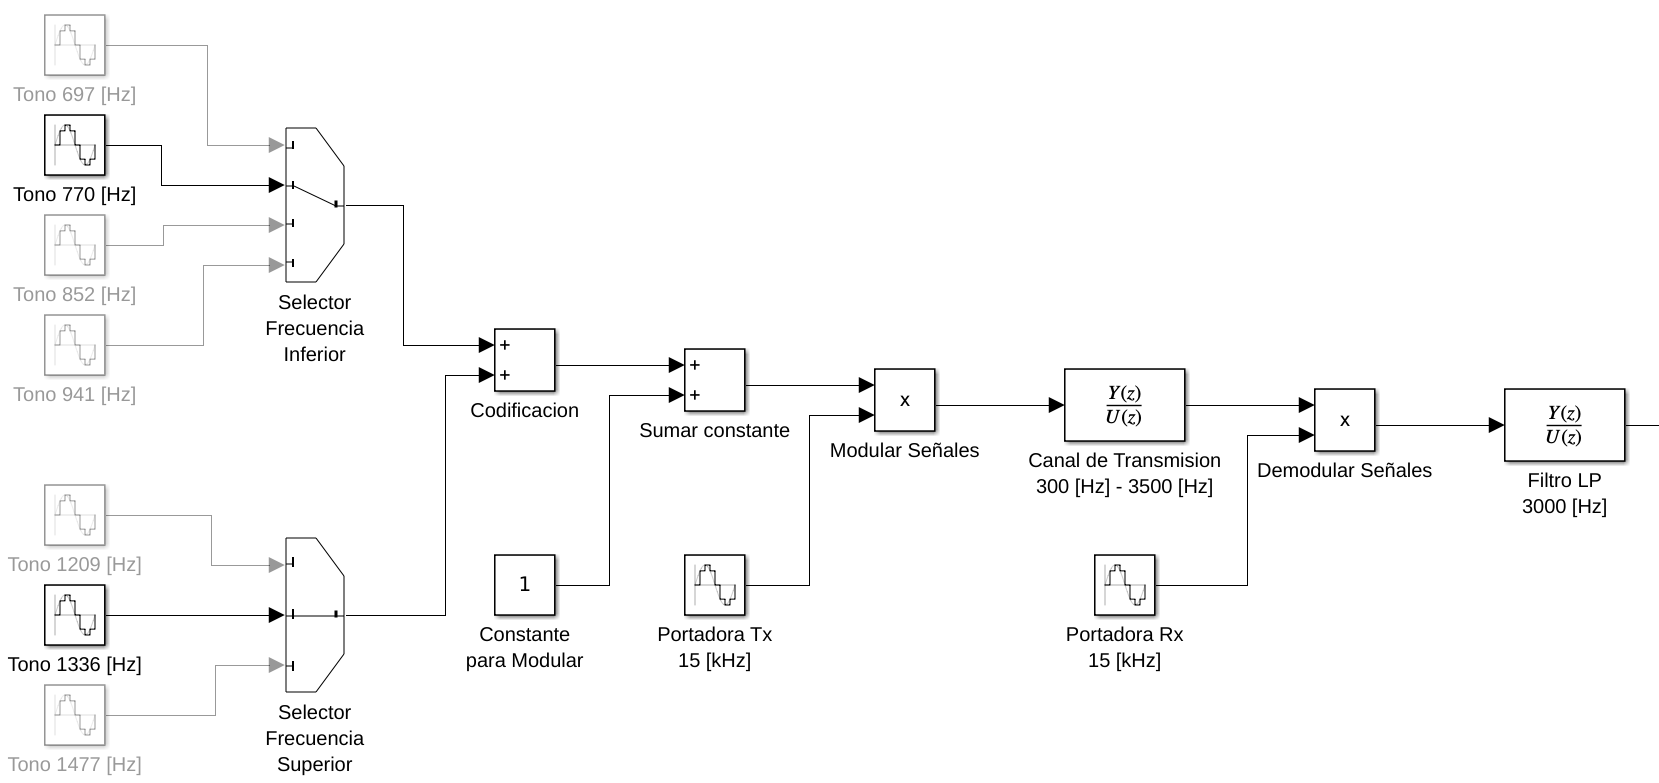
\includegraphics[width=\linewidth]{images/modem.png}
  \caption{Codificación, Modulación, Transmisión y Demodulación}
  \label{fig:bloques_modem}
\end{figure}

\begin{figure}[H]
  \centering
  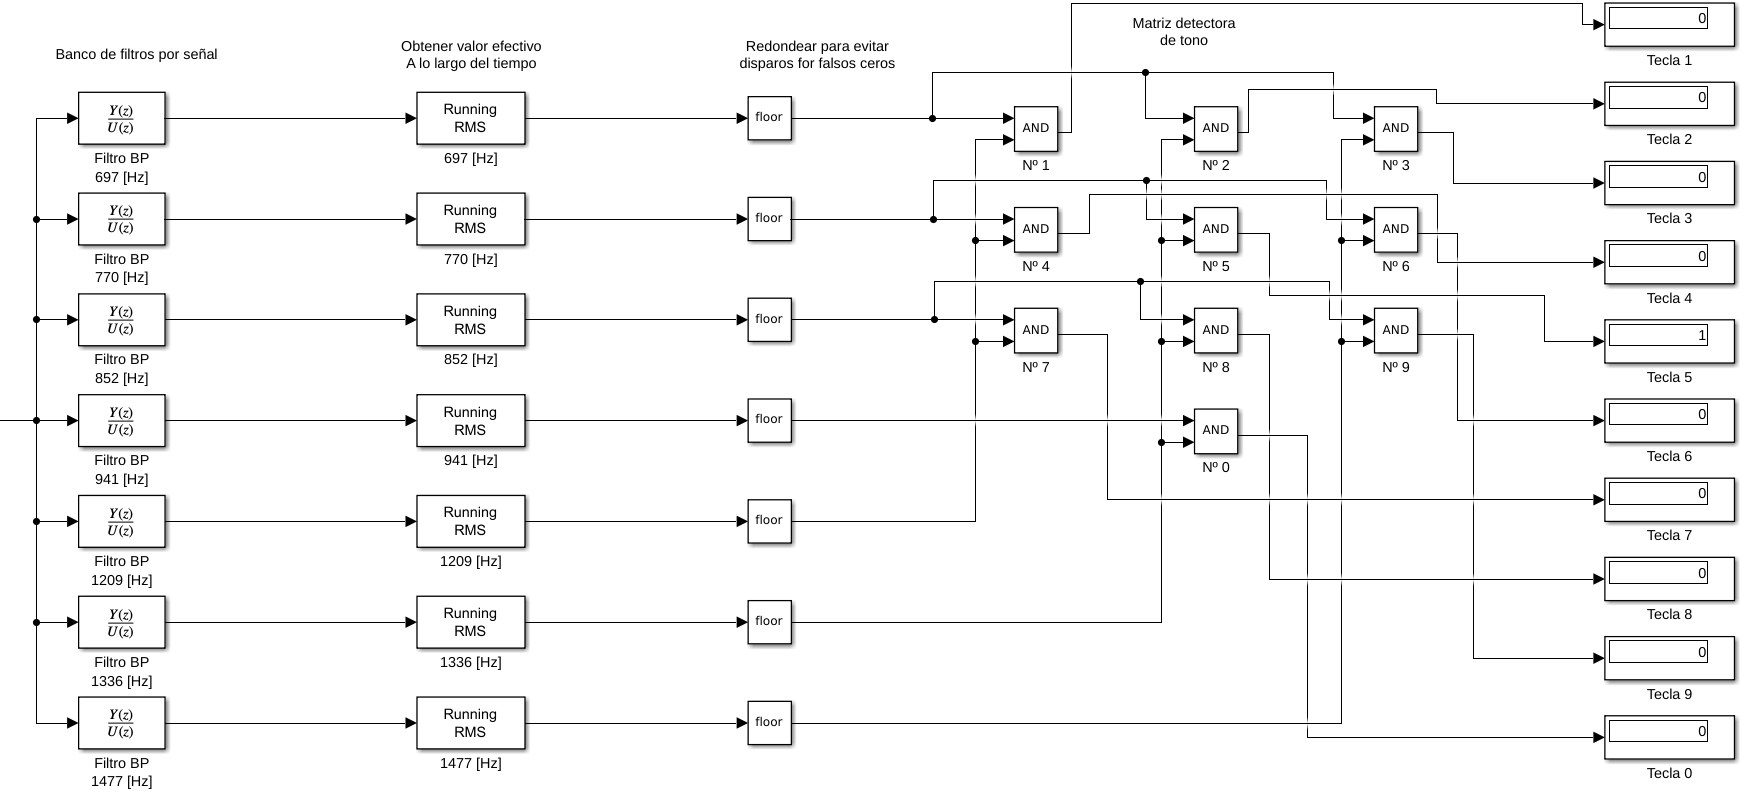
\includegraphics[width=\linewidth]{images/codec.png}
  \caption{Banco de filtros y Decodificador}
  \label{fig:bloques_codec}
\end{figure}

La matriz decodificadora se compone de bloques de operación lógica AND. La salida de este bloque será 1 si y solo si ambas entradas son diferentes a 0\footnote{En el álgebra booleana aplicada en sistemas de control, todo valor igual a 0 se toma como "Falso", mientras que cualquier valor distinto de 0, por más infinitesimal que sea, es "Verdadero"}. Como los filtros anteriores son de orden relativamente bajo, es posible que al tratar las señales dejen pasar vestigios de la otra señal en la codificación pero con mucha menor amplitud. El valor efectivo de este resultado puede ser muy bajo, infinitesimal, del orden de $10^{-2}$, pero no 0 y por consiguiente el operador lógico lo tomará como válido y puede disparar falsos valores. Por esa razón debemos tomar la parte entera del valor eficaz, para garantizar que solo se debe tomar como válida a las señales que realmente son de la misma frecuencia que la frecuencia central de cada filtro.

\section{Simulación}
Para llevar a cabo la simulación vamos a considerar una serie de escenarios posibles, en los que se diferencia mayormente la confiabilidad en el canal de transmisión. Es decir, confiaremos en los bloques de control ya que son implementados a través de sistemas computacionales, pero el medio de transmisión es analógico y su eficacia depende de muchos factores físicos. Este se puede ver alterado de diversas maneras haciendo que parte de la información se pierda o corrompa. Para ello vamos a probar los siguientes escenarios:

\begin{enumerate}
  \item El canal de transmisión es del tipo AWG-24 de menos de 200 [m] de largo, cuyo ancho de banda es de 1 [MHz].
  \item El canal de transimsión es extenso y tiene el ancho de banda del espectro audíble por los humanos.
  \item El mismo canal anterior presenta fallas atenuando en diferentes frecuencias dentro del espectro de tonos \gls{dtfm}
\end{enumerate}

\subsection{Ancho de banda Extendido - 1 [MHz]}
\subsection{Ancho de banda Reducido - 3 [kHz]}
\subsection{Canal con Fallas}